% Chinese support

\documentclass[a4paper,twoside]{ctexart}
\usepackage{blindtext}  
\usepackage{geometry}


\ctexset{
	section={
		format+ = \zihao{-3} \heiti \raggedright,
		number = \chinese{section}
	}
}

% Page margin layout
\geometry{left=2.3cm,right=2cm,top=2.5cm,bottom=2.0cm}


\usepackage{listings}
\usepackage{xcolor}
\usepackage{geometry}
\usepackage{amsmath}
\usepackage{float}
\usepackage{hyperref}

\usepackage{graphics}
\usepackage{graphicx}
\usepackage{subfigure}
\usepackage{epsfig}
\usepackage{float}

\usepackage{circuitikz}
\usepackage{pbox}
\usepackage{bbding}
\usepackage{karnaugh-map}
\newcommand{\ctikzlabel}[2]{\pbox{\textwidth}{#1\\#2}}


\usepackage{algorithm}
\usepackage[noend]{algpseudocode}

\usepackage{booktabs}
\usepackage{threeparttable}
\usepackage{longtable}
\usepackage{listings}
\usepackage{tikz}
\usepackage{multicol}

% cite package, to clean up citations in the main text. Do not remove.
\usepackage{cite}

\usepackage{color,xcolor}

%% The amssymb package provides various useful mathematical symbols
\usepackage{amssymb}
%% The amsthm package provides extended theorem environments
\usepackage{amsthm}
\usepackage{amsfonts}
\usepackage{enumerate}
\usepackage{enumitem}
\usepackage{listings}

\usepackage{pdfpages}

\usepackage{indentfirst}
\setlength{\parindent}{2em} % Make two letter space in the first paragraph
\usepackage{setspace}
\linespread{1.5} % Line spacing setting
\usepackage{siunitx}
\setlength{\parskip}{0.5em} % Paragraph spacing setting

% \usepackage[contents =22920202204622, scale = 10, color = black, angle = 50, opacity = .10]{background}

\renewcommand{\figurename}{图}
\renewcommand{\lstlistingname}{代码} 
\renewcommand{\tablename}{表格}
\renewcommand{\contentsname}{目录}
\floatname{algorithm}{算法}

\graphicspath{ {images/} }

%%%%%%%%%%%%%
\newcommand{\StudentNumber}{22920202204622}  % Fill your student number here
\newcommand{\StudentName}{熊恪峥}  % Replace your name here
\newcommand{\PaperTitle}{数字逻辑实验(五)、实验(六)}  % Change your paper title here
\newcommand{\PaperType}{实验报告} % Replace the type of your report here
\newcommand{\Date}{2022年5月8日}
\newcommand{\College}{信息学院}
\newcommand{\CourseName}{数字逻辑}
%%%%%%%%%%%%%

%% Page header and footer setting
\usepackage{fancyhdr}
\usepackage{lastpage}
\pagestyle{fancy}
\fancyhf{}
% This requires the document to be twoside
\fancyhead[LO]{\texttt{\StudentName }}
\fancyhead[LE]{\texttt{\StudentNumber}}
\fancyhead[C]{\texttt{\PaperTitle }}
\fancyhead[R]{\texttt{第{\thepage}页,共\pageref*{LastPage}页}}


\title{\PaperTitle}
\author{\StudentName}
\date{\Date}

\lstset{
	basicstyle          =   \sffamily,          % 基本代码风格
	keywordstyle        =   \bfseries,          % 关键字风格
	commentstyle        =   \rmfamily\itshape,  % 注释的风格,斜体
	stringstyle         =   \ttfamily,  % 字符串风格
	flexiblecolumns,                % 别问为什么,加上这个
	numbers             =   left,   % 行号的位置在左边
	showspaces          =   false,  % 是否显示空格,显示了有点乱,所以不现实了
	numberstyle         =   \zihao{-5}\ttfamily,    % 行号的样式,小五号,tt等宽字体
	showstringspaces    =   false,
	captionpos          =   t,      % 这段代码的名字所呈现的位置,t指的是top上面
	frame               =   lrtb,   % 显示边框
}

\lstdefinestyle{PythonStyle}{
	language        =   Python, % 语言选Python
	basicstyle      =   \zihao{-5}\ttfamily,
	numberstyle     =   \zihao{-5}\ttfamily,
	keywordstyle    =   \color{blue},
	keywordstyle    =   [2] \color{teal},
	stringstyle     =   \color{magenta},
	commentstyle    =   \color{red}\ttfamily,
	breaklines      =   true,   % 自动换行,建议不要写太长的行
	columns         =   fixed,  % 如果不加这一句,字间距就不固定,很丑,必须加
	basewidth       =   0.5em,
}

\algnewcommand\algorithmicinput{\textbf{Input:}}
\algnewcommand\algorithmicoutput{\textbf{Output:}}
\algnewcommand\Input{\item[\algorithmicinput]}%
\algnewcommand\Output{\item[\algorithmicoutput]}%

\usetikzlibrary{positioning, shapes.geometric}

\newcommand{\ols}[1]{\mskip.5\thinmuskip\overline{\mskip-.5\thinmuskip {#1} \mskip-.5\thinmuskip}\mskip.5\thinmuskip}

% \usepackage{draftwatermark}
% \SetWatermarkText{22920202204622}
% \SetWatermarkScale{0.8}

\begin{document}
	
%%%%%%%%%%%%%%%%%%%%%%%%%%%%%%%%%%%%%%%%%%%%
\makeatletter % change default title style
\renewcommand*\maketitle{%
	\begin{center} 
		\bfseries  % title 
		{\LARGE \@title \par}  % LARGE typesetting
		\vskip 1em  %  margin 1em
		{\global\let\author\@empty}  % no author information
		{\global\let\date\@empty}  % no date
		\thispagestyle{empty}   %  empty page style
	\end{center}%
	\setcounter{footnote}{0}%
}
\makeatother
%%%%%%%%%%%%%%%%%%%%%%%%%%%%%%%%%%%%%%%%%%%%
	
	
\thispagestyle{empty}

\vspace*{1cm}

\begin{figure}[h]
	\centering
	\includegraphics[width=4.0cm]{logo.png}
\end{figure}

\vspace*{1cm}

\begin{center}
	\Huge{\textbf{\PaperType}}
	
	\Large{\PaperTitle}
\end{center}

\vspace*{1cm}

\begin{table}[h]
	\centering	
	\begin{Large}
		\renewcommand{\arraystretch}{1.5}
		\begin{tabular}{p{3cm} p{5cm}<{\centering}}
			姓\qquad 名 & \StudentName  \\
			\hline
			学\qquad号 & \StudentNumber \\
			\hline
			日\qquad期 & \Date  \\
			\hline
			学\qquad院 & \College  \\
			\hline
			课程名称 & \CourseName  \\
			\hline
		\end{tabular}
	\end{Large}
\end{table}

\newpage

\title{
	\Large{\textcolor{black}{\PaperTitle}}
}
 
\newpage
\setcounter{page}{1}

\begin{spacing}{1.2}

\includepdf[pages={11,12,13,14}]{../instruction.pdf}
\setcounter{section}{4}

\section{实验结果}

\subsection{消除抖动}

通过示波器观察可以发现脉冲博兴较为稳定。

\subsection{RC环形震荡器}

搭建如图所示的电路,使用$1k\Omega$电阻作为$R$,用示波器测的震荡的周期和频率如表~\ref{tbl:rc}

\begin{table}[htbp]
	\centering
	\caption{震荡周期和频率}
	\label{tbl:rc}
	\begin{tabular}{c|ccccc}
		\toprule
		\hline
		C & $0.1\mu$ & $0.022\mu$ & $0.01\mu$ & $1000p$ & $100p$ \\
		\hline
		T & 0.00022 & $\num{4.84e-05}$ & $\num{2.2e-05}$ & $\num{2.2e-6}$ & $\num{2.2e-07}$ \\ 
		\hline
		f & $4545.455$& $20661.16$ & $45454.5$ & $454544.5$ & $4545452$ \\
		\hline
		\bottomrule 
	\end{tabular}	
\end{table}

可见基本符合公式$T=2.2RC$

\subsection{集成D触发器}

按题目要求测量,得到表~\ref{tbl:dtg}。

\begin{table}[htbp]
	\centering
	\caption{D触发器}
	\label{tbl:dtg}
	\begin{tabular}{c|c|c|c}
		\toprule
		\hline
		D & CP & $Q^n$& $Q^{n+1}$ \\
		\hline
		0 & $\uparrow$ & 0 & 0 \\
		0 & $\uparrow$ & 1 & 0 \\
		0 & $\downarrow$ & 0 & 0 \\
		0 & $\downarrow$ & 1 & 1 \\
		1 & $\uparrow$ & 0 & 1 \\
		1 & $\uparrow$ & 1 & 1 \\
		1 & $\downarrow$ & 0 & 0 \\
		1 & $\downarrow$ & 1 & 1 \\
		\hline
		\bottomrule
	\end{tabular}
\end{table}

\subsection{集成JK触发器}

测试$S_D$、$R_D$的作用,得到表~\ref{tbl:jksr}。

\begin{table}[htbp]
	\centering
	\caption{JK触发器$S_D$、$R_D$的作用}
	\label{tbl:jksr}
	\begin{tabular}{c|c|c|c|c|c|c}
		\toprule
		\hline
		CP & J & K & $S_D$ & $R_D$ & $Q$ & $\ols{Q}$ \\
		\hline
		$\times$ & $\times$ & $\times$ & 1 & 0 & 0 & 1 \\
		$\times$ & $\times$ & $\times$ & 0 & 1 & 1 & 0 \\
		\hline
		\bottomrule
	\end{tabular}
\end{table}

测试JK触发器的逻辑功能,得到表~\ref{tbl:jk}

\begin{table}[H]
	\centering
	\caption{JK触发器}
	\label{tbl:jk}
	\begin{tabular}{cc|c|cc}
		\toprule
		\hline
		J & K & CP & $Q^n$& $Q^{n+1}$ \\
		\hline
		0 & 0 & $\uparrow$ & 0 & 0 \\
		0 & 0 & $\uparrow$ & 1 & 1 \\
		0 & 0 & $\downarrow$ & 0 & 0 \\
		0 & 0 & $\downarrow$ & 1 & 1 \\
		\hline
		0 & 1 & $\uparrow$ & 0 & 0 \\
		0 & 1 & $\uparrow$ & 1 & 0 \\
		0 & 1 & $\downarrow$ & 0 & 0 \\
		0 & 1 & $\downarrow$ & 1 & 1 \\
		\hline
		1 & 0 & $\uparrow$ & 0 & 1 \\
		1 & 0 & $\uparrow$ & 1 & 1 \\
		1 & 0 & $\downarrow$ & 0 & 0 \\
		1 & 0 & $\downarrow$ & 1 & 1 \\
		\hline
		1 & 1 & $\uparrow$ & 0 & 1 \\
		1 & 1 & $\uparrow$ & 1 & 0 \\
		1 & 1 & $\downarrow$ & 0 & 0 \\
		1 & 1 & $\downarrow$ & 1 & 1 \\
		\hline
		\bottomrule
	\end{tabular}
\end{table}

可见符合JK触发器的状态方程。

\subsection{D触发器和JK触发器的相互转换}

根据题目中所给的图片连接电路,测试到的结果与表~\ref{tbl:jk}和表~\ref{tbl:dtg}相符。
可见转换结果是正确的。

\section{实验总结}

通过该实验,我测试了D触发器和JK触发器的逻辑功能,并且实现了D触发器和JK触发器的相互转换。
对触发器的功能和转换得到了更好的理解。

\clearpage

\includepdf[pages={15,16}]{../instruction.pdf}
\setcounter{section}{4}

\section{电路设计}

\subsection{移位寄存器型计数器电路}

根据电路图和D触发器可以写出激励函数\eqref{eqn:exct1}。

\begin{equation}
\label{eqn:exct1}
\begin{aligned}
	Q_4^{(n+1)}&=Q_3 \\
	Q_3^{(n+1)}&=Q_2 \\
	Q_2^{(n+1)}&=Q_1 \\
	Q_1^{(n+1)}&=\ols{\ols{\ols{Q_3\cdot \ols{Q_1}} \cdot \ols{Q_4}}} \\
	&=\ols{Q_3\cdot \ols{Q_1}} \cdot \ols{Q_4}
\end{aligned}
\end{equation}

可以画出状态图如图~\ref{fig:dfn1}

\begin{figure}[htbp]
	\centering
	\caption{状态图}
	\label{fig:dfn1}
	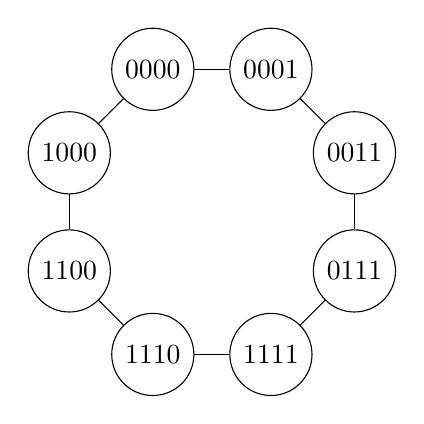
\begin{tikzpicture}[node distance={15mm},main/.style = {draw, circle}] 
		\node[main] (0) [] {$0000$};
		\node[main] (1) [right of=0] {$0001$};
		\node[main] (3) [below right of=1] {$0011$}; 
		\node[main] (7) [below of=3] {$0111$};
		\node[main] (15) [below left of=7] {$1111$}; 
		\node[main] (14) [left of=15] {$1110$};
		\node[main] (12) [above left of=14] {$1100$};
		\node[main] (8) [above of=12] {$1000$};
		\draw (0) to (1);
		\draw (1) to (3);
		\draw (3) to (7);
		\draw (7) to (15);
		\draw (15) to (14);
		\draw (14) to (12);
		\draw (12) to (8);
		\draw (8) to (0);
	\end{tikzpicture}
\end{figure}

并写出状态表如表~\ref{tbl:stable1}

\begin{table}[htbp]
	\centering
	\caption{状态表}
	\label{tbl:stable1}
	\begin{tabular}{cccc|cccc|cccc}
		\toprule
		\hline
		$Q_4$&$Q_3$&$Q_2$&$Q_1$&$D_4$&$D_3$&$D_2$&$D_1$&$Q_4^{(n+1)}$&$Q_3^{(n+1)}$&$Q_2^{(n+1)}$&$Q_1^{(n+1)}$ \\
		\hline
		0&0&0&0&0&0&0&1&0&0&0&1 \\
		0&0&0&1&0&0&1&1&0&0&1&1 \\
		0&0&0&1&0&0&1&1&0&0&1&1 \\
		0&0&1&1&0&1&1&1&0&1&1&1 \\
		0&1&1&1&1&1&1&1&1&1&1&1 \\
		1&1&1&1&1&1&1&0&1&1&1&0 \\
		1&1&1&0&1&1&0&0&1&1&0&0 \\
		1&1&0&0&1&0&0&0&1&0&0&0 \\
		1&0&0&0&0&0&0&0&0&0&0&0 \\
		\hline
		\bottomrule
	\end{tabular}
\end{table}

可以画出电路图电路图如图~\ref{fig:51}

\begin{figure}[htbp]
	\centering
	\caption{电路图}
	\label{fig:51}
	\includegraphics[width=0.48\textwidth]{51.png}
\end{figure}

\clearpage

\subsection{同步模5计数器}

需要输出BCD码的同步模5计数器,首先画出状态图,如图~\ref{fig:dfn2}。

\begin{figure}[htbp]
	\centering
	\caption{状态图}
	\label{fig:dfn2}

	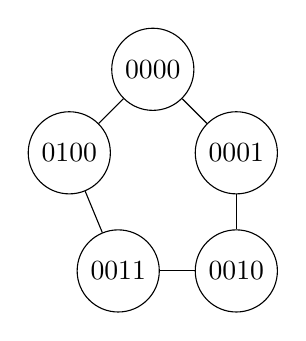
\begin{tikzpicture}[node distance={15mm},main/.style = {draw, circle}] 
		\node[main] (0) [] {$0000$};
		\node[main] (1) [below right of=0] {$0001$};
		\node[main] (2) [below of=1] {$0010$}; 
		\node[main] (3) [left of=2] {$0011$};
		\node[main] (4) [below left of=0] {$0100$}; 
		\draw (0) to (1);
		\draw (1) to (2);
		\draw (2) to (3);
		\draw (3) to (4);
		\draw (4) to (0);
	\end{tikzpicture}
\end{figure}

可见最高位恒为0,则需要用3个D触发器。因此写出状态表,如表~\ref{tbl:stable2}。

\begin{table}[htbp]
	\centering
	\caption{状态表}
	\label{tbl:stable2}
	\begin{tabular}{ccc|ccc|ccc}
		\toprule
		\hline
		$Q_3$&$Q_2$&$Q_1$&$Q_3^{(n+1)}$&$Q_2^{(n+1)}$&$Q_1^{(n+1)}$&$D_3$&$D_2$&$D_1$ \\
		\hline
		0&0&0&0&0&1&0&0&1 \\
		0&0&1&0&1&0&0&1&0 \\
		0&1&0&0&1&1&0&1&1 \\
		0&1&1&1&0&0&1&0&0 \\
		1&0&0&0&0&0&0&0&0 \\
		\hline
		\bottomrule
	\end{tabular}
\end{table}

根据该表写出逻辑表达式\eqref{eqn:exct2}

\begin{equation}
	\label{eqn:exct2}
	\begin{aligned}
		D_3&=\ols{Q_3}\cdot Q_2\cdot Q_1 \\
		D_2&=\ols{Q_3}\cdot\ols{Q_2}\cdot Q_1 + \ols{Q_3}\cdot Q_2\cdot\ols{Q_1} \\
		&= \ols{\ols{\ols{Q_3}\cdot(Q_2 \oplus Q_1)}} \\
		D_1&=\ols{Q_3}\cdot\ols{Q_2}\cdot\ols{Q_1} \\
	\end{aligned}
\end{equation}

根据以上表达式可以画出电路图如图~\ref{fig:53}

\begin{figure}[htbp]
	\centering
	\caption{电路图}
	\label{fig:53}
	\includegraphics[width=0.48\textwidth]{53.png}
\end{figure}

\clearpage

\subsection{模10计数器}

要显示计数值,需要输出BCD码的同步模10计数器,因此采用反馈清零法。态序表如表~\ref{tbl:sseq1}。

\begin{table}[htbp]
	\centering
	\caption{态序表}
	\label{tbl:sseq1}
	\begin{tabular}{c|cccc}
		\toprule
		\hline
		$N$&$Q_D$&$Q_C$&$Q_B$&$Q_A$ \\
		\hline
		0&0&0&0&0 \\
		1&0&0&0&1 \\
		2&0&0&1&0 \\
		3&0&0&1&1 \\
		4&0&1&0&0 \\
		5&0&1&0&1 \\
		6&0&1&1&0 \\
		7&0&1&1&1 \\
		8&1&0&0&0 \\
		9&1&0&0&1 \\
		\hline
		\bottomrule
	\end{tabular}
\end{table}

当$Q_DQ_CQ_BQ_A=1001$时进行清零。清零信号为$C_r=\ols{Q_D\ols{Q_C}\ols{Q_B}Q_A}$

根据以上清零表达式可以画出电路图如图~\ref{fig:54}

\begin{figure}[htbp]
	\centering
	\caption{电路图}
	\label{fig:54}
	\includegraphics[width=0.48\textwidth]{54.png}
\end{figure}

\clearpage

\section{实验结果}

\subsection{移位寄存器型计数器电路}

按预习报告连接电路,测试状态如表~\ref{tbl:res61}。可见结果是正确的。

\begin{table}[htbp]
	\centering
	\caption{状态表}
	\label{tbl:res61}
	\begin{tabular}{ccc|ccc|ccc}
		\toprule
		\hline
		$Q_3$&$Q_2$&$Q_1$&$Q_3^{(n+1)}$&$Q_2^{(n+1)}$&$Q_1^{(n+1)}$&$D_3$&$D_2$&$D_1$ \\
		\hline
		0&0&0&0&0&1&0&0&1 \\
		0&0&1&0&1&0&0&1&0 \\
		0&1&0&0&1&1&0&1&1 \\
		0&1&1&1&0&0&1&0&0 \\
		1&0&0&0&0&0&0&0&0 \\
		\hline
		\bottomrule
	\end{tabular}
\end{table}

连接电路实物图如图~\ref{fig:res61}

\begin{figure}[htbp]
	\centering
	\caption{实物图}
	\label{fig:res61}
	\includegraphics[width=0.48\textwidth,angle=90]{61.jpg}
\end{figure}

\subsection{同步模5计数器}

按预习报告连接电路,测试状态如表~\ref{tbl:res62}。可见结果是正确的。

\begin{table}[htbp]
	\centering
	\caption{实验结果}
	\label{tbl:res62}
	\begin{tabular}{ccc|ccc|ccc}
		\toprule
		\hline
		$Q_3$&$Q_2$&$Q_1$&$Q_3^{(n+1)}$&$Q_2^{(n+1)}$&$Q_1^{(n+1)}$&$D_3$&$D_2$&$D_1$ \\
		\hline
		0&0&0&0&0&1&0&0&1 \\
		0&0&1&0&1&0&0&1&0 \\
		0&1&0&0&1&1&0&1&1 \\
		0&1&1&1&0&0&1&0&0 \\
		1&0&0&0&0&0&0&0&0 \\
		\hline
		\bottomrule
	\end{tabular}
\end{table}

\clearpage

\subsection{同步模10计数器}
按预习报告连接电路,测试状态如表~\ref{tbl:res63}。可见结果是正确的。

\begin{table}[htbp]
	\centering
	\caption{实验结果}
	\label{tbl:res64}
	\begin{tabular}{c|cccc}
		\toprule
		\hline
		$N$&$Q_D$&$Q_C$&$Q_B$&$Q_A$ \\
		\hline
		0&0&0&0&0 \\
		1&0&0&0&1 \\
		2&0&0&1&0 \\
		3&0&0&1&1 \\
		4&0&1&0&0 \\
		5&0&1&0&1 \\
		6&0&1&1&0 \\
		7&0&1&1&1 \\
		8&1&0&0&0 \\
		9&1&0&0&1 \\
		\hline
		\bottomrule
	\end{tabular}
\end{table}

连接电路实物图如图~\ref{fig:res63}

\begin{figure}[htbp]
	\centering
	\caption{实物图}
	\label{fig:res63}
	\includegraphics[width=0.48\textwidth,angle=90]{63.jpg}
\end{figure}

\subsection{实验总结}

本实验使用分立门电路、集成电路实现了计数器。通过这次实验我学习到了在设计计数器
时,化简表达式的结果是否足够简单对搭建电路有重要的意义,同时也练习了搭建复杂电路
的技巧。

\end{spacing}

\end{document}